%%%%%%%%%%%%%%%%%%%%%%%%%%%%%%%%%%%%%%%%%
% University/School Laboratory Report
% LaTeX Template
% Version 3.1 (25/3/14)
%
% This template has been downloaded from:
% http://www.LaTeXTemplates.com
%
% Original author:
% Linux and Unix Users Group at Virginia Tech Wiki
% (https://vtluug.org/wiki/Example_LaTeX_chem_lab_report)
%
% License:
% CC BY-NC-SA 3.0 (http://creativecommons.org/licenses/by-nc-sa/3.0/)
%
%%%%%%%%%%%%%%%%%%%%%%%%%%%%%%%%%%%%%%%%%

%----------------------------------------------------------------------------------------
%	PACKAGES AND DOCUMENT CONFIGURATIONS
%----------------------------------------------------------------------------------------

\documentclass{article}

\usepackage{graphicx} % Required for the inclusion of images
\usepackage{minted}

\setlength\parindent{0pt} % Removes all indentation from paragraphs

\renewcommand{\labelenumi}{\alph{enumi}.} % Make numbering in the enumerate environment by letter rather than number (e.g. section 6)

%\usepackage{times} % Uncomment to use the Times New Roman font

%----------------------------------------------------------------------------------------
%	DOCUMENT INFORMATION
%----------------------------------------------------------------------------------------

\title{In the name of God \\ Database Lab \\ Spring 2016} % Title

\author{Iman \textsc{Tabrizian}} % Author name

\date{\today} % Date for the report

\begin{document}

\maketitle % Insert the title, author and date

\begin{center}
	\begin{tabular}{l r}
		Date Performed: & April 6, 2016 \\ % Date the experiment was performed
		Partners: & Parham Alvani \\ % Partner names
	\end{tabular}
\end{center}

% If you wish to include an abstract, uncomment the lines below
% \begin{abstract}
% Abstract text
% \end{abstract}

%----------------------------------------------------------------------------------------
%	SECTION 1
%----------------------------------------------------------------------------------------

\section{Results and Conclusions}
\begin{enumerate}
	\item
		\inputminted{sql}{sql/impar-1.sql}
	\item
		\inputminted{sql}{sql/impar-1-a.sql}
	\item
		\inputminted{sql}{sql/impar-1-exec.sql}
	\item
		\inputminted{sql}{sql/impar-1-select.sql}
	\item
		\inputminted{sql}{sql/impar-1-upgrade.sql}
	\item
		\inputminted{sql}{sql/impar-2-exec.sql}
	\item
		\inputminted{sql}{sql/impar-3.sql}
	\item
		\inputminted{sql}{sql/impar-3-exec.sql}
	\item
		\inputminted{sql}{sql/impar-4.sql}
	\item
		\inputminted{sql}{sql/impar-4-1.sql}
	\item
		\inputminted{sql}{sql/impar-5.sql}
	\item
		\inputminted{sql}{sql/impar-6.sql}
	\item
		\inputminted{sql}{sql/impar-6-exec.sql}
	\item
		\inputminted{sql}{sql/impar-7.sql}
\end{enumerate}
\section{Screen Shots}
\begin{enumerate}
	\item
		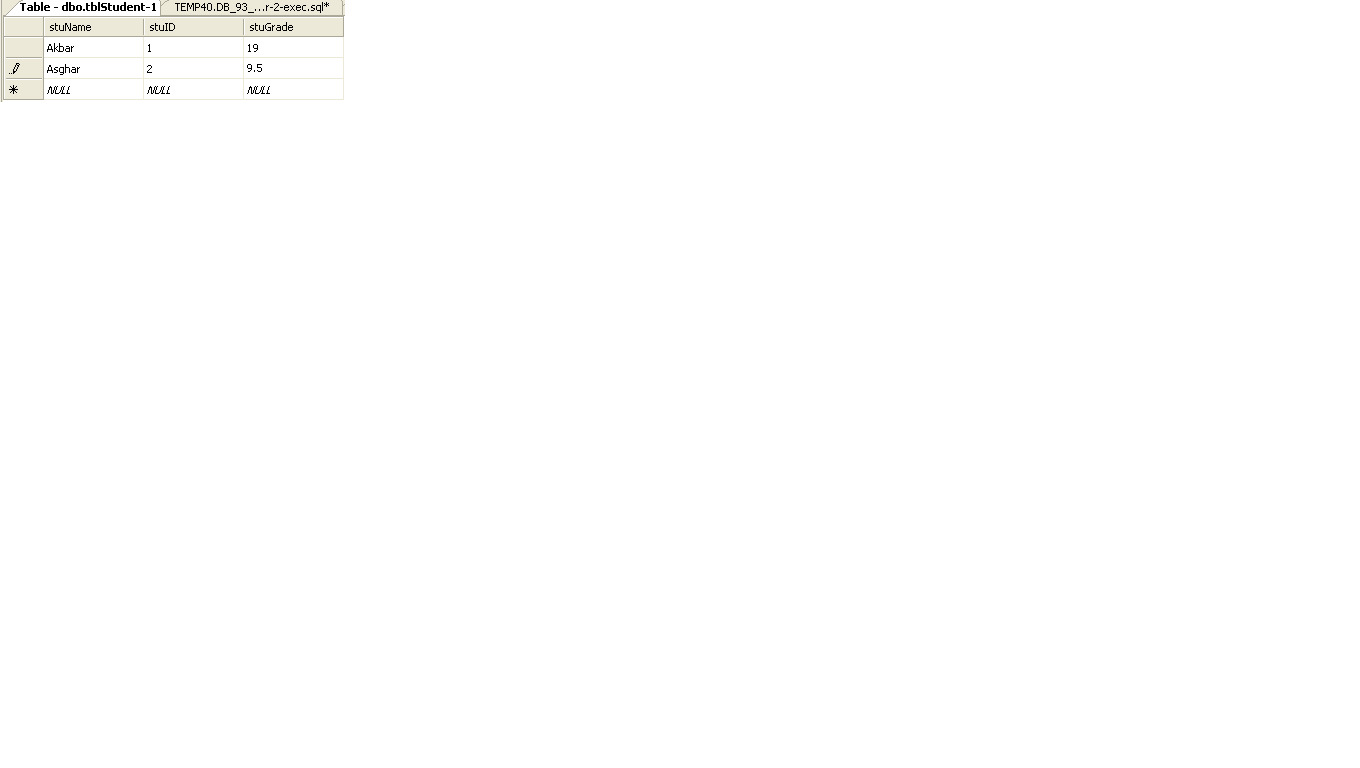
\includegraphics[scale=0.5]{figs/im-2.jpg}
	\item
		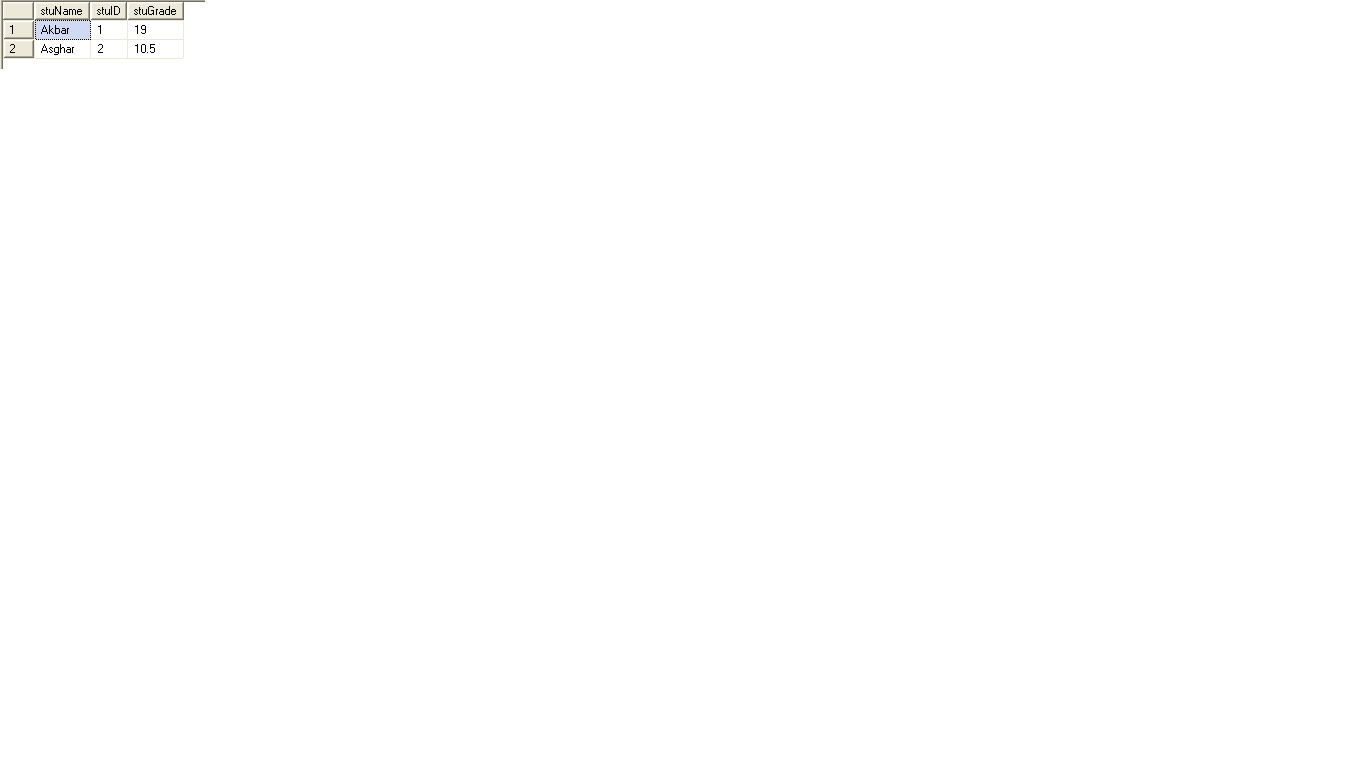
\includegraphics[scale=0.5]{figs/im-2-2.jpg}
	\item
		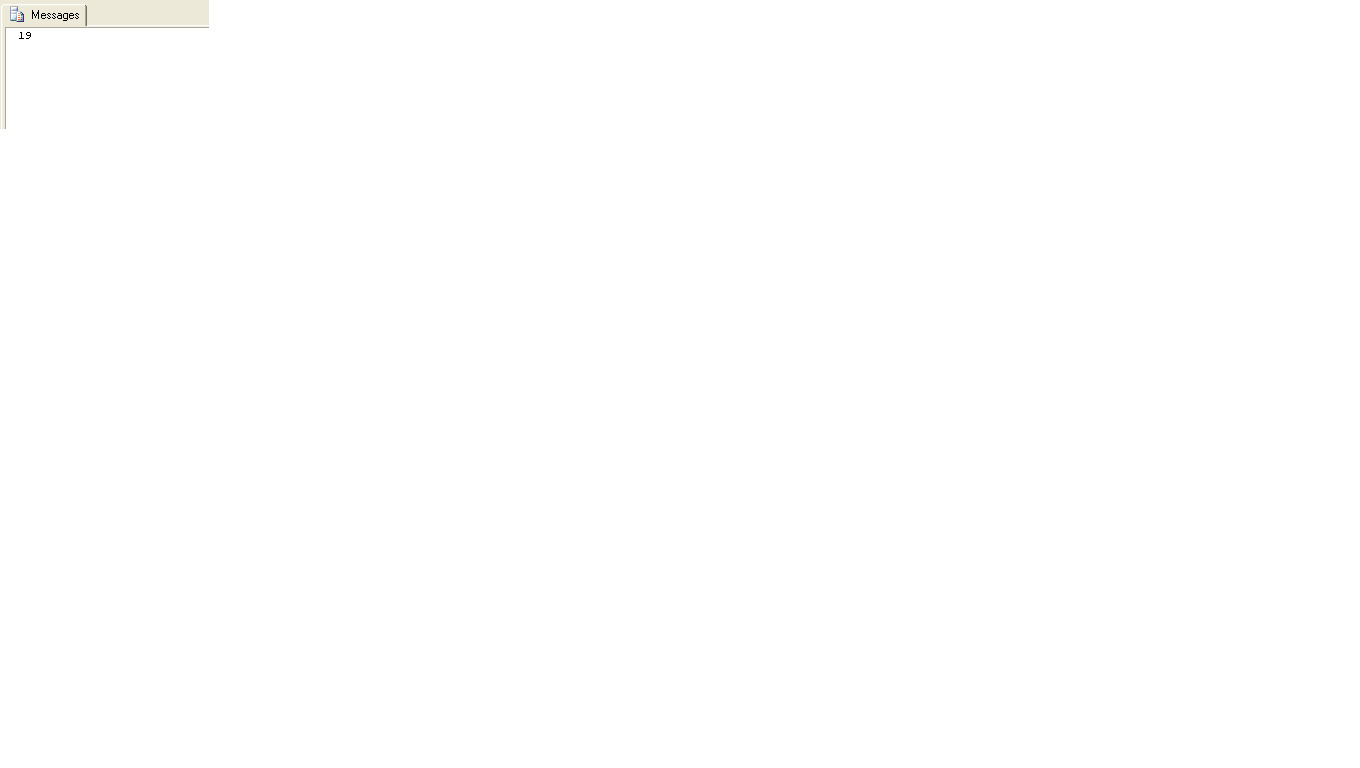
\includegraphics[scale=0.5]{figs/im-4.jpg}
	\item
		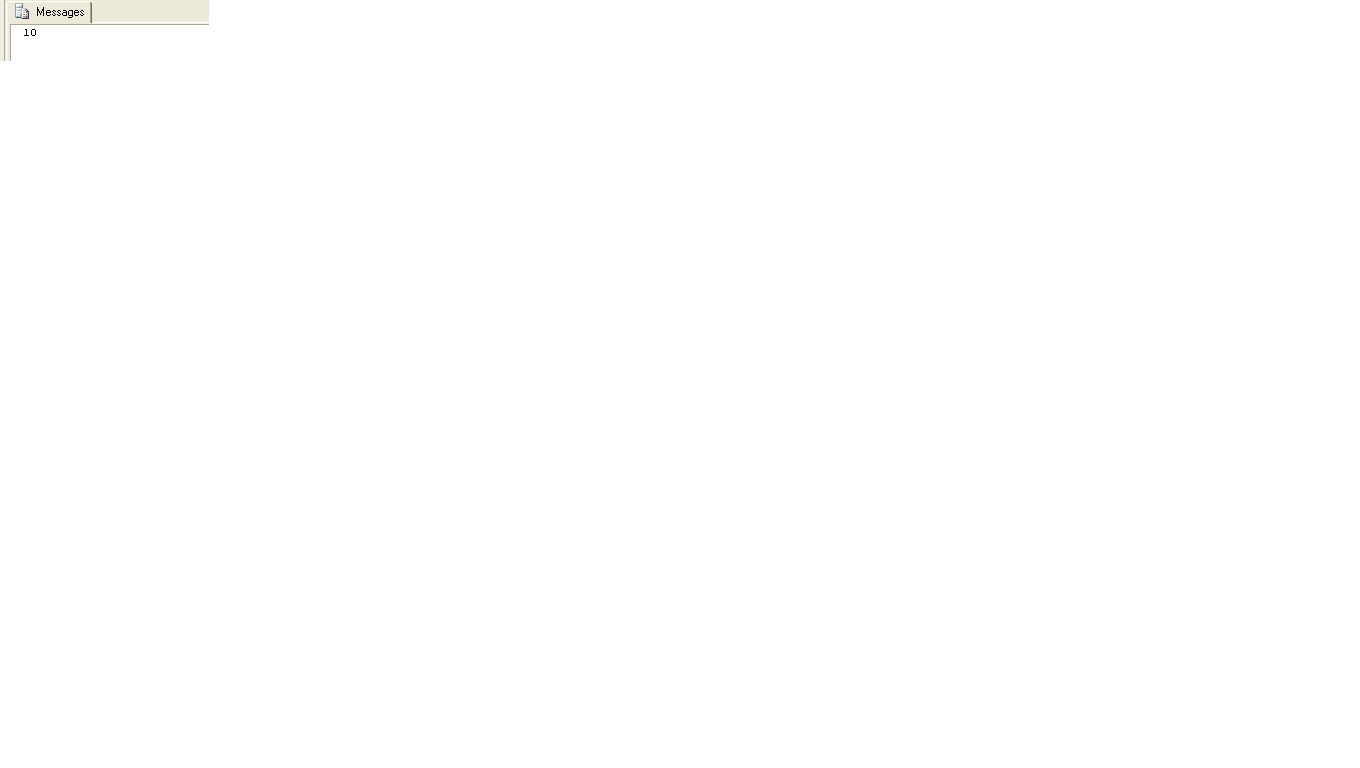
\includegraphics[scale=0.5]{figs/im-6-exec.jpg}
	\item
		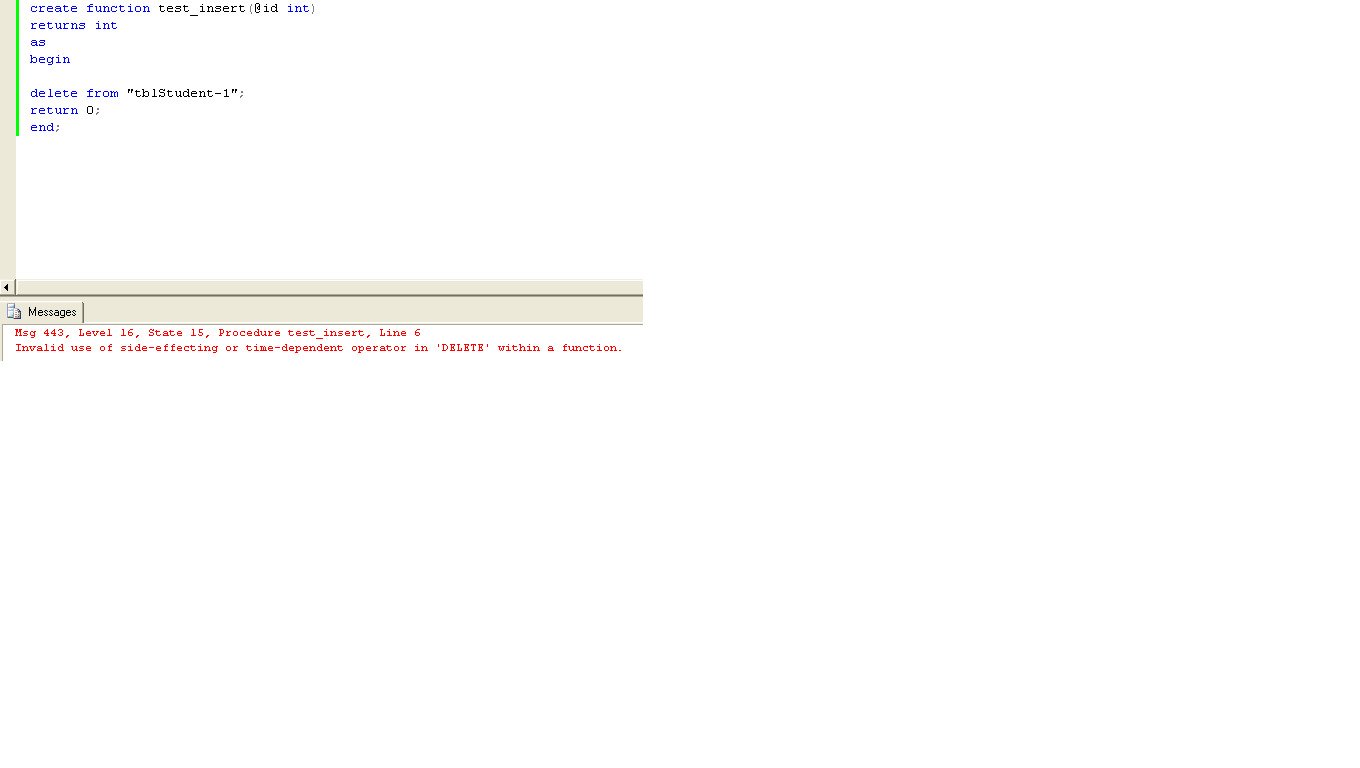
\includegraphics[scale=0.5]{figs/im-7-exec-delete.jpg}
	\item
		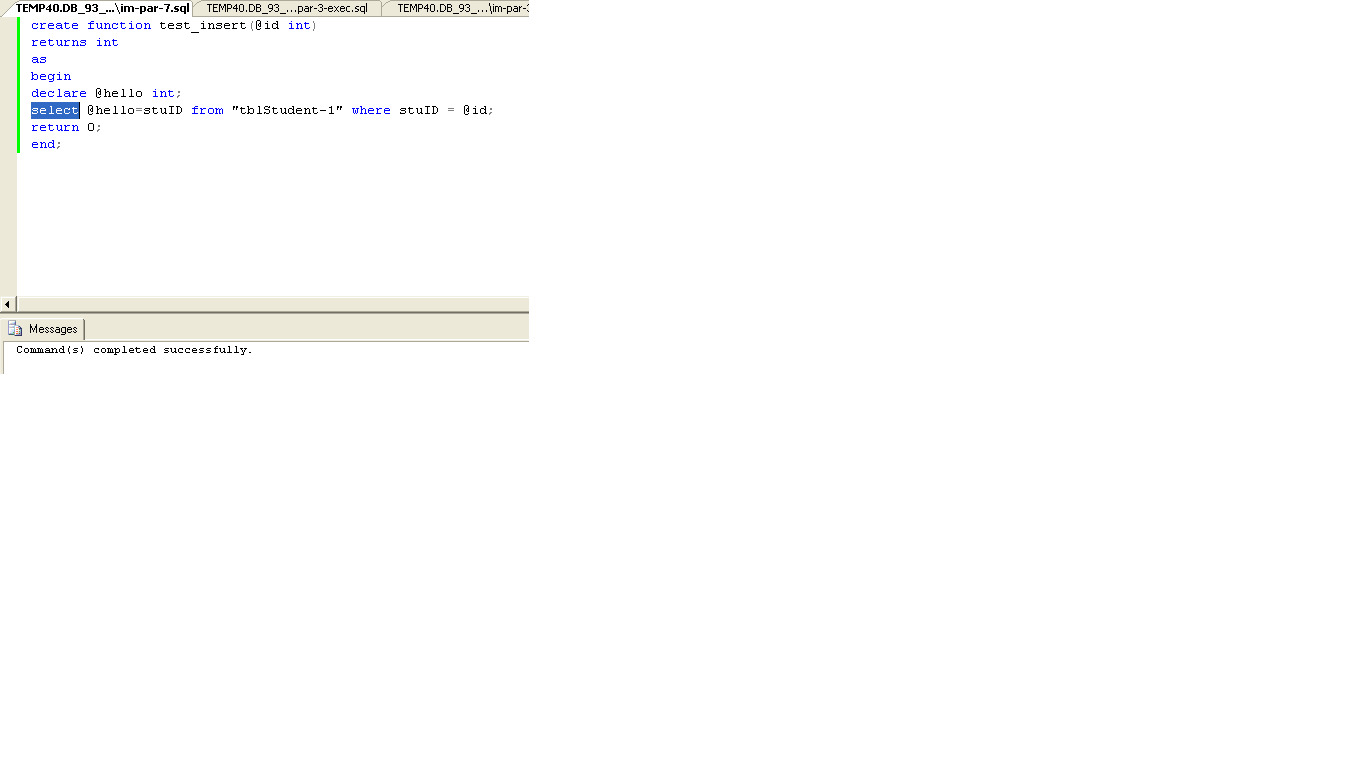
\includegraphics[scale=0.5]{figs/im-7-exec-select.jpg}
	\item
		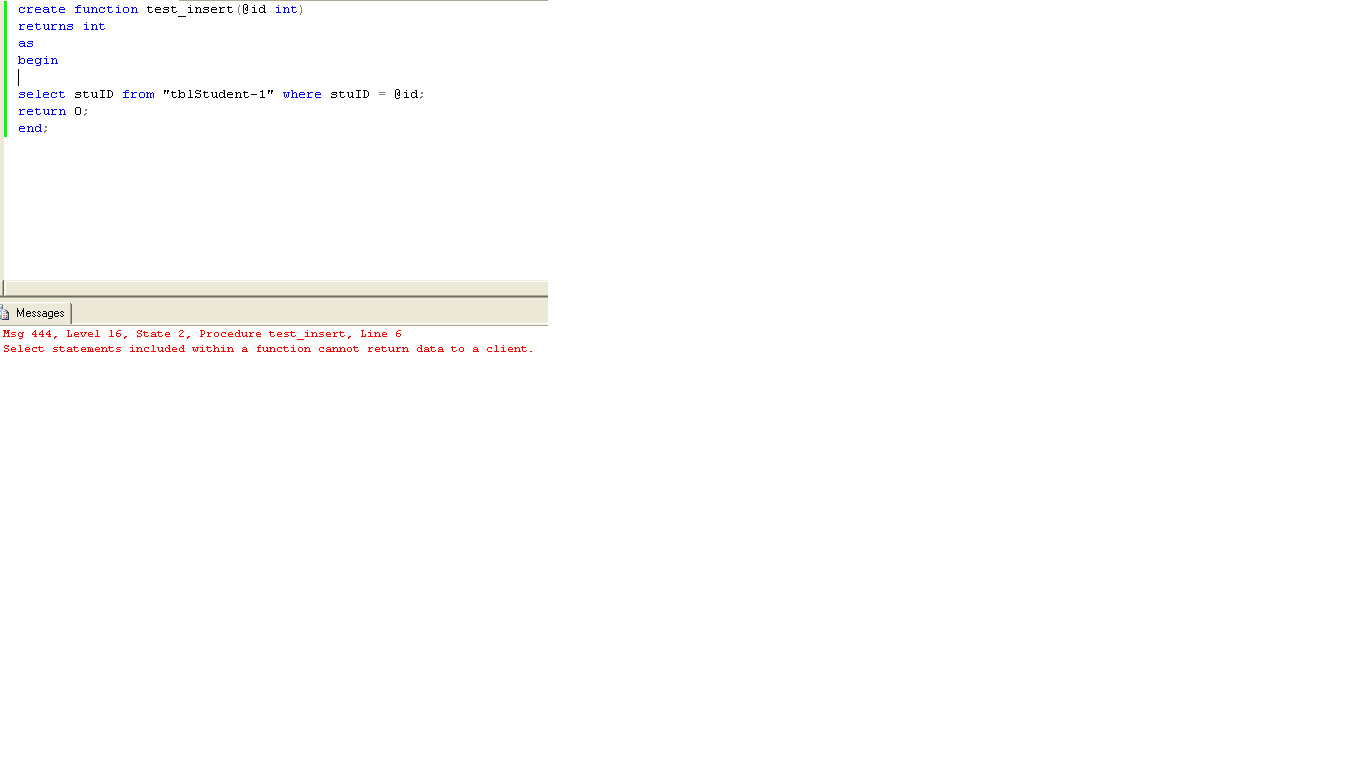
\includegraphics[scale=0.5]{figs/im-7-exec-select-error.jpg}
	\item
		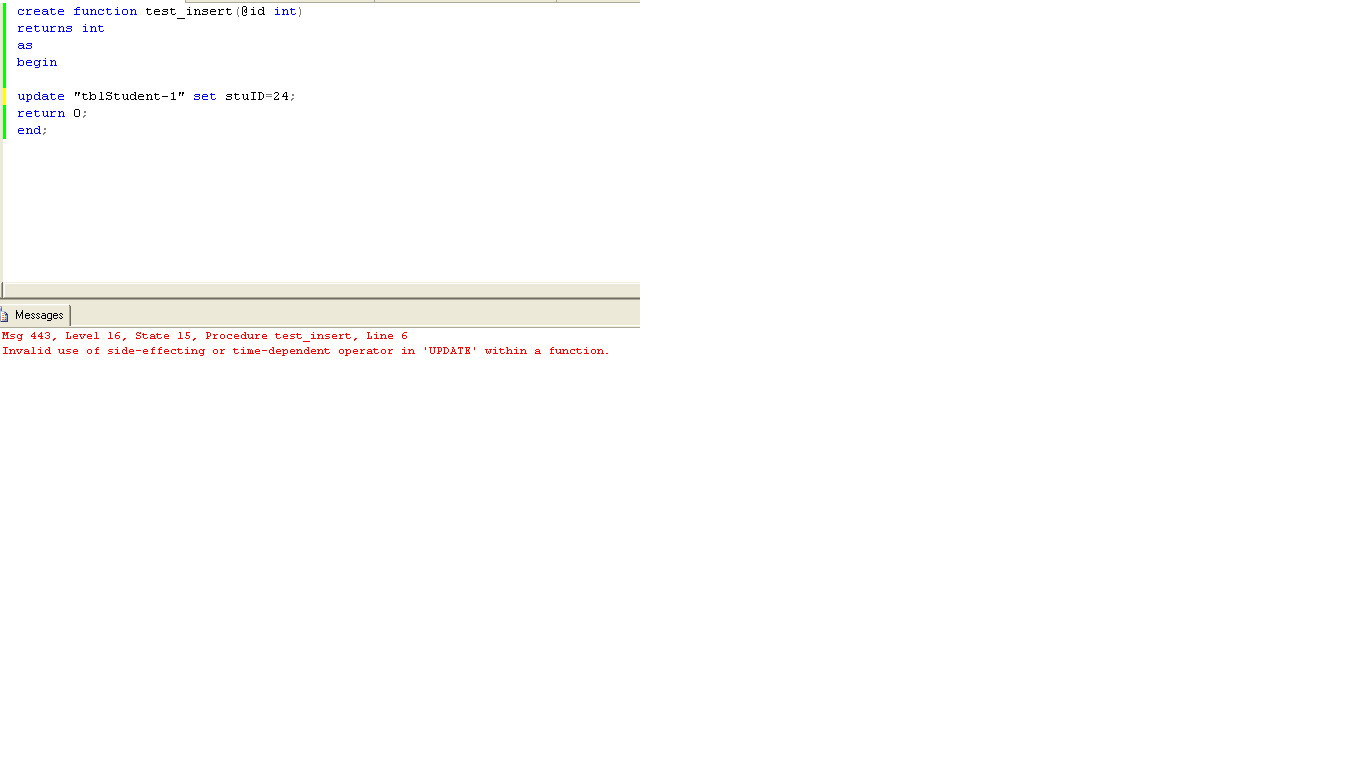
\includegraphics[scale=0.5]{figs/im-7-exec-update.jpg}
\end{enumerate}
\end{document}
